\documentclass[10pt,a4paper]{article}

\usepackage[margin=2.2cm]{geometry}
\usepackage[utf8]{inputenc}
\usepackage[T1]{fontenc}
\usepackage{lmodern}
\usepackage{amsmath,amssymb}
\usepackage{booktabs}
\usepackage{array}
\usepackage{tabularx}
\usepackage{enumitem}
\usepackage{graphicx}
\usepackage{xcolor}
\usepackage{listings}
\usepackage{microtype}
\usepackage{tikz}
\usepackage{hyperref}
\usepackage{caption}
\usepackage{titlesec}
\usepackage{algorithm}
\usepackage{algpseudocode}

\usetikzlibrary{arrows.meta,positioning,fit,backgrounds,calc}
\hypersetup{
  colorlinks=true,
  linkcolor=blue!50!black,
  urlcolor=blue!50!black,
  citecolor=blue!50!black
}
\setlist[itemize]{leftmargin=1.3em,itemsep=2pt,topsep=3pt}
\setlist[enumerate]{leftmargin=1.5em,itemsep=2pt,topsep=3pt}
\titleformat{\section}{\large\bfseries}{\thesection}{0.8em}{}
\titleformat{\subsection}{\normalsize\bfseries}{\thesubsection}{0.7em}{}
\newcommand{\pres}{\mathrm{pres}}
\newcommand{\on}{\mathrm{on}}
\newcommand{\off}{\mathrm{off}}
\newcommand{\IoU}{\mathrm{IoU}}
\newcommand{\PSDS}{\mathrm{PSDS}}
\newcommand{\Softplus}{\operatorname{Softplus}}
\newcommand{\median}{\operatorname{median}}

\title{\textbf{Technical Report}\\[4pt]
Sound Event Detection with\\Boundary-Aware Optimization and Inference}
\author{Le Duc Minh\\
\texttt{minh.leduc.0210@gmail.com}\\
Reproduction and analysis of arXiv:2601.04178}
\date{November 24, 2026}

\begin{document}
\maketitle

\begin{abstract}
This report explains the paper \emph{Sound Event Detection with Boundary-Aware
Optimization and Inference} \cite{paper} (Schmid et al., arXiv:2601.04178) and the
reproduction in this repository. It covers the Recurrent Event Detection (RED)
layer, the Onset--Offset Loss (OOL), Event Proposal Networks (EPN), the event
inference algorithm, the training objective, and the PSDS1/PSDS2/collar-F1
metrics. It then describes a CRNN reproduction on URBAN-SED, reports measured
results, and evaluates capacity, augmentation, post-processing and ensemble
extensions. The best single model reaches 45.77 PSDS1; a post-hoc four-model
ensemble reaches 47.73, an optimistic upper bound. The report is written
to be readable without prior sound event detection background.
\end{abstract}

\tableofcontents

\section{The problem: sound event detection}

Sound event detection (SED) takes an audio clip and returns a set of events
\begin{equation}
\mathcal{E} = \{(c_j,\; t^{\mathrm{start}}_j,\; t^{\mathrm{end}}_j)\},
\end{equation}
where $c_j$ is the event class and the two timestamps are its boundaries.

There are two common designs. \emph{Event-based} systems directly predict a set
of events, but need complex objectives such as Hungarian matching.
\emph{Frame-wise} systems predict, for every class $c$ and frame $t$, a
probability that the event is active:
\begin{equation}
\hat p^{\pres}_{c,t} = P(e_{c,t}=1).
\end{equation}
Frame-wise models are the dominant paradigm because they train well with
multiple-instance learning and simple architectures such as a convolutional
recurrent neural network (CRNN), and they work with weakly labelled data.

Their weakness is converting frame probabilities into events. The standard
recipe is: (i) smooth the probability curve, usually with a median filter;
(ii) threshold it; (iii) group consecutive active frames into events. The filter
length and threshold are tuned on a validation set after training. This
post-processing is non-differentiable and can discard information the model
learned. The paper's goal is to remove that separate tuning step by learning
event boundaries and proposals inside the model.


\section{Background and related work}

SED research has two broad lines. Frame-wise systems predict a probability per
class and frame. Early work paired convolutional features with recurrent layers
\cite{cakir2017}, added gating \cite{xu2018}, or used dilated convolutions
\cite{li2020}. These models train with weak clip labels through multiple-instance
learning \cite{kumar2016,wang2019} and remain the backbone of current DCASE
systems. Event-based systems predict a set of intervals directly
\cite{venkatesh2022,ye2021,bhosale2024}. They avoid post-processing but need
complex assignment rules such as Hungarian matching, and their training is less
stable on small datasets.

Frame-wise outputs still need a decision rule. Median filtering is the standard
choice in DCASE baselines \cite{turpault2019}. Sound event bounding boxes (SEBB)
\cite{ebbers2024} and hidden semi-Markov models (HSM3) \cite{yoshinaga2025}
improve on median filtering, but both add a separate inference stage with
hyperparameters tuned after training. The paper studied here replaces that stage
with learned proposals.

The datasets shape the problem. DESED \cite{turpault2019} mixes real and
synthetic domestic recordings. AudioSet Strong \cite{hershey2021} provides
strong labels at web scale. URBAN-SED \cite{salamon2017urbansed} synthesises
10-second urban scenes from UrbanSound8K clips \cite{salamon2014}; it is small
enough for a single GPU and has clean strong labels, which makes it useful for
method studies. General introductions to the task and its metrics appear in
\cite{mesaros2021,virtanen2018}.

Architecture choices matter as much as the temporal layer. Frequency dynamic
convolution (FDY) \cite{nam2022fdy} adapts kernels across frequency bands.
Audio transformers such as ATST \cite{li2024atst} and BEATs
\cite{chen2023beats} provide strong pretrained representations. Efficient CNN
and CRNN variants \cite{morocutti2025} trade accuracy for speed. Conformer and
multi-resolution systems \cite{barahona2023} improve long-range modelling.
Training recipes add mixup \cite{zhang2018mixup}, SpecAugment
\cite{park2019specaugment}, Freq-MixStyle \cite{kim2022freqmix} and
FilterAugment \cite{nam2022filteraug}; semi-supervised variants use consistency
training \cite{tarvainen2017}.

Evaluation has moved from threshold-dependent event F1 to PSDS
\cite{bilen2020}. The threshold-independent formulation of Ebbers et al.
\cite{ebbers2022} is now standard, and later work studies evaluation without
post-processing \cite{ebbers2023}. This report reports PSDS1, PSDS2 and
collar-F1, and treats PSDS1 as the primary localisation metric.

\section{Overview of the proposed method}

The method keeps a standard frame-wise acoustic model but changes what the model
predicts and how events are extracted.

\begin{figure}[t]
\centering
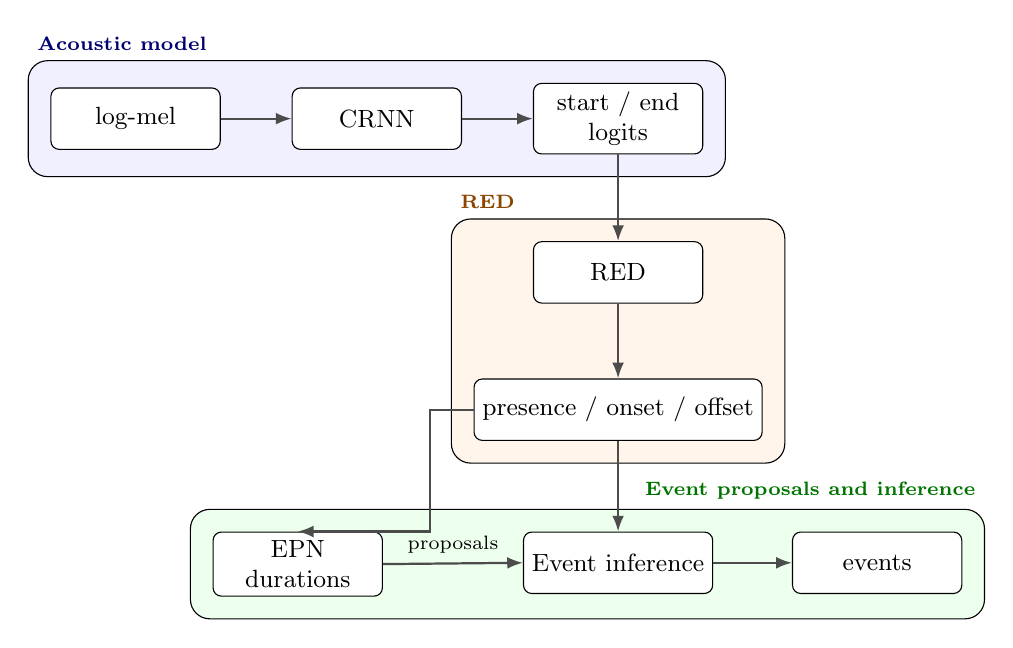
\begin{tikzpicture}[
  node distance=8mm and 9mm,
  box/.style={draw, rounded corners=3pt, fill=white, minimum width=2.15cm,
              minimum height=0.78cm, align=center, font=\small, inner sep=3pt},
  group/.style={draw, rounded corners=7pt, inner sep=8pt},
  arr/.style={-{Latex[length=2mm]}, thick, draw=black!70}
]
\node[box] (mel) {log-mel};
\node[box, right=of mel] (crnn) {CRNN};
\node[box, right=of crnn] (logits) {start / end\\logits};
\node[box, below=1.1cm of logits] (red) {RED};
\node[box, below=0.95cm of red] (probs) {presence / onset / offset};
\node[box, below left=1.15cm and 1.15cm of probs] (epn) {EPN\\durations};
\node[box, below=1.15cm of probs] (infer) {Event inference};
\node[box, right=1.0cm of infer] (events) {events};

\draw[arr] (mel) -- (crnn);
\draw[arr] (crnn) -- (logits);
\draw[arr] (logits) -- (red);
\draw[arr] (red) -- (probs);
\draw[arr] (probs.south) -- (infer.north);
\draw[arr] (probs.west) -- ++(-0.55,0) |- (epn.north);
\draw[arr] (epn.east) -- node[above, font=\scriptsize] {proposals} (infer.west);
\draw[arr] (infer.east) -- (events.west);


\begin{scope}[on background layer]
  \node[group, fill=blue!6, fit=(mel)(crnn)(logits)] (g1) {};
  \node[group, fill=orange!8, fit=(red)(probs)] (g2) {};
  \node[group, fill=green!7, fit=(epn)(infer)(events)] (g3) {};
  \node[anchor=south west, font=\scriptsize\bfseries, text=blue!45!black]
       at (g1.north west) {Acoustic model};
  \node[anchor=south west, font=\scriptsize\bfseries, text=orange!55!black]
       at (g2.north west) {RED};
  \node[anchor=south east, font=\scriptsize\bfseries, text=green!45!black]
       at (g3.north east) {Event proposals and inference};
\end{scope}
\end{tikzpicture}
\caption{Pipeline of the boundary-aware SED method. The acoustic model emits
start and end logits; RED turns them into presence/onset/offset probabilities;
EPN predicts a duration interval per frame; the event inference step selects
proposals and returns events. The training objectives are BCE on presence, focal loss on
onset/offset, and the duration-weighted IoU loss on proposals.}
\label{fig:pipeline}
\end{figure}

Three components are added:
\begin{enumerate}
\item \textbf{RED} turns conditional start/end probabilities into presence,
      onset and offset probabilities.
\item \textbf{OOL} applies focal losses to the sparse onset/offset labels.
\item \textbf{EPN} predicts a time interval around each frame and replaces
      median filtering with a proposal-selection algorithm.
\end{enumerate}
The acoustic model outputs two logits per class per frame: a start logit and an
end logit.

\section{RED: Recurrent Event Detection}

\subsection{Notation}
For one class, let
\begin{itemize}
\item $e_t\in\{0,1\}$ be the event-presence variable at frame $t$;
\item $s_t=P(e_t=1\mid e_{t-1}=0)$ be the conditional start probability;
\item $z_t=P(e_t=0\mid e_{t-1}=1)$ be the conditional end probability;
\item $p_t=P(e_t=1)$ be the presence probability.
\end{itemize}
The model produces start and end logits; a sigmoid gives $s_t$ and $z_t$.

\subsection{The recurrence}
Assume $p_{-1}=0$. Presence at $t$ can come from two cases: an event starts at
$t$ (probability $s_t$, previous frame inactive with probability $1-p_{t-1}$),
or an event was active and does not end at $t$ (probability $1-z_t$, previous
frame active with probability $p_{t-1}$). Therefore
\begin{equation}
\boxed{p_t = s_t(1-p_{t-1}) + (1-z_t)p_{t-1}}.
\end{equation}
The onset and offset probabilities are
\begin{equation}
\mathrm{onset}_t = s_t(1-p_{t-1}),
\qquad
\mathrm{offset}_t = z_t p_{t-1}.
\end{equation}
Presence rises at onsets and falls at offsets, while remaining smooth
elsewhere.

\subsection{Why it is cheap}
Rewrite the recurrence as an affine scan:
\begin{equation}
p_t = a_t p_{t-1} + b_t,
\qquad
a_t = 1-s_t-z_t,
\qquad
b_t = s_t.
\end{equation}
Affine recurrences compose associatively:
\begin{equation}
(a_1,b_1)\circ(a_2,b_2)
=
(a_2a_1,\; a_2b_1+b_2).
\end{equation}
This permits a parallel prefix scan in $O(\log T)$ sequential steps instead of
$T$ Python iterations. The implementation uses a Hillis--Steele scan \cite{heinsen2023}; a sequential
reference is kept for tests. RED has no learnable parameters.

\subsection{Why this helps}
The acoustic model no longer learns one presence curve directly. It learns two
simpler conditional ``switch'' signals: when an event starts and when it ends.
Presence is derived deterministically. The onset and offset outputs are
temporally localised peaks, exactly what the boundary losses can supervise.


\section{OOL: Onset--Offset Loss}

Ground-truth onset and offset labels are derived from annotations:
$y^{\on}_{c,t}=1$ on the first frame of each event, $y^{\off}_{c,t}=1$ on the
first frame after each event, and zero elsewhere. These labels are extremely
sparse: a 10-second clip has only a handful of boundary frames out of 500.
Plain BCE would be dominated by negatives, so the paper uses a focal loss with
focusing exponent $2$ (the paper writes this as $\alpha=2$; in the focal-loss
literature the exponent is usually $\gamma$):
\begin{equation}
\mathcal{L}_{\on/\off}
=
-\frac{1}{CT}
\sum_{c=1}^{C}\sum_{t=1}^{T}
\begin{cases}
(1-\hat p_{c,t})^{\alpha}\log \hat p_{c,t}, & y_{c,t}=1,\\[3pt]
\hat p_{c,t}^{\alpha}\log(1-\hat p_{c,t}), & y_{c,t}=0.
\end{cases}
\end{equation}
The implementation computes both terms separately:
\begin{equation}
\mathcal{L}_{\mathrm{ool}}
=
\mathcal{L}_{\on}+\mathcal{L}_{\off}.
\end{equation}
For a positive boundary frame with low predicted probability, the factor
$(1-\hat p)^2$ is near one and the loss is large. For an easy negative with low
probability, $\hat p^2$ is tiny and the loss is suppressed. Because RED couples
presence, onset and offset, these losses also shape the presence curve.


\section{EPN: Event Proposal Network}

\subsection{Duration prediction}
EPN takes the three RED outputs per class and frame,
$[\hat p^{\pres}_{c,t},\hat p^{\on}_{c,t},\hat p^{\off}_{c,t}]$, and predicts
two non-negative durations:
\begin{align}
\hat d^{\on}_{c,t} &= \Softplus(h^{\on}_{c,t}),\\
\hat d^{\off}_{c,t} &= \Softplus(h^{\off}_{c,t}),
\end{align}
where $h$ is the output of a bidirectional GRU followed by a linear layer.
The proposal for frame $t$ is
\begin{equation}
\hat r_{c,t}
=
[t-\hat d^{\on}_{c,t},\; t+\hat d^{\off}_{c,t}].
\end{equation}
Two variants exist: \emph{per-class GRUs} (one GRU per class, input
$[0,1]^{3\times T}$) and a \emph{single GRU} over all classes (input
$[0,1]^{3C\times T}$). The per-class variant is used for AS-Strong-10; the
single-GRU variant is used for many classes. Both are implemented.

\subsection{IoU loss}
For a frame inside an event, the ground-truth interval is
\begin{equation}
r_{c,t}
=
[t-d^{\on}_{c,t},\; t+d^{\off}_{c,t}].
\end{equation}
Both $r_{c,t}$ and $\hat r_{c,t}$ contain $t$, so intersection and union have a
closed form:
\begin{equation}
\IoU_{c,t}
=
\frac{
\min(d^{\on}_{c,t},\hat d^{\on}_{c,t})
+
\min(d^{\off}_{c,t},\hat d^{\off}_{c,t})
}{
\max(d^{\on}_{c,t},\hat d^{\on}_{c,t})
+
\max(d^{\off}_{c,t},\hat d^{\off}_{c,t})
}.
\end{equation}
The loss is evaluated on active frames and weighted by ground-truth duration:
\begin{equation}
\mathcal{L}_{\mathrm{iou}}
=
\frac{1}{\sum_{c,t} y^{\pres}_{c,t}}
\sum_{c,t}
y^{\pres}_{c,t}
\left(1-\IoU_{c,t}\right)
\left(d^{\on}_{c,t}+d^{\off}_{c,t}\right).
\end{equation}
\begin{algorithm}[t]
\caption{Duration-weighted IoU loss for one batch}
\label{alg:iou}
\begin{algorithmic}[1]
\Require predicted $\hat d^{\on},\hat d^{\off}$; targets $d^{\on},d^{\off}$;
         presence labels $y^{\pres}$
\State $inter \gets \min(\hat d^{\on},d^{\on})+\min(\hat d^{\off},d^{\off})$
\State $union \gets \max(\hat d^{\on},d^{\on})+\max(\hat d^{\off},d^{\off})$
\State $iou \gets inter / \max(union,\epsilon)$ \Comment{$\epsilon=10^{-7}$}
\State $weight \gets d^{\on}+d^{\off}$
\State $L \gets \sum y^{\pres}(1-iou)\,weight
       \big/ \max(\sum y^{\pres},1)$
\State \Return $L$
\end{algorithmic}
\end{algorithm}

The implementation follows the algebra in Algorithm~\ref{alg:iou}. Both
intervals contain $t$, so the intersection and union reduce to sums of minima
and maxima; no interval sorting is needed. The duration factor weights every active frame by the length of its event, so
longer events contribute more to the sum than shorter ones. This is not an
equal-per-event weighting; it is the form used in the paper, where it was more
stable than direct duration regression. In our URBAN-SED runs the weight
mattered: $\lambda_{\mathrm{iou}}=2$ gave 25.87 PSDS1, while $0.5$ gave 35.42.
The paper tunes this value per backbone. On URBAN-SED the choice moves PSDS1 by
about 9.5 points, which is larger than the gain the method was meant to deliver;
$\lambda_{\mathrm{iou}}=4$ was not run, and no cross-dataset transfer claim is
made.


\section{Event inference}

Algorithm~\ref{alg:infer} (Algorithm~1 of the paper) replaces thresholding and
median filtering. Inputs are the presence
probabilities $\hat p^{\pres}_{c,t}$, proposals $\hat r_{c,t}$, a maximum
$k$ events per class (default 15), and the $m$ most active classes (default all).
For each selected class:
\begin{enumerate}
\item sort frames by presence;
\item take the unprocessed frame $t$ with the highest presence; its proposal
      $\hat r_{c,t}$ is the candidate;
\item set its event score $\sigma$ to the mean presence over the proposal;
\item emit $(c,\;t-\hat d^{\on},\;t+\hat d^{\off},\;\sigma)$;
\item suppress every proposal overlapping the chosen interval;
\item repeat until $k$ events or no proposals remain.
\end{enumerate}
This is a non-maximum-suppression-like procedure. It is not differentiable; it
only converts learned proposals into a final event set.

The baseline is the usual frame-wise post-processing:
\begin{equation}
\tilde p_t
=
\median\left(p_{t-\lfloor L/2\rfloor},\ldots,p_{t+\lfloor L/2\rfloor}\right),
\end{equation}
followed by threshold $\tau$ and grouping of consecutive active frames.

\begin{algorithm}[t]
\caption{Event inference (Algorithm~1 of the paper)}
\label{alg:infer}
\begin{algorithmic}[1]
\Require presence $\hat p^{\pres}_{c,t}$; proposals $\hat r_{c,t}$;
         max events per class $k$; max classes $m$
\Ensure event set $\mathcal{E}$
\State $s_c \gets \operatorname{mean}_t \hat p^{\pres}_{c,t}$ for every class
\State select the $m$ classes with the largest $s_c$
\State $\mathcal{E} \gets \emptyset$
\For{each selected class $c$}
  \State order frames by $\hat p^{\pres}_{c,t}$ descending
  \State $removed_t \gets \mathrm{false}$ for all $t$
  \State $\mathcal{E}_c \gets \emptyset$ \Comment{events selected for class $c$}
  \For{$t$ in that order}
    \If{$removed_t$ or $|\mathcal{E}_c| \ge k$}
      \State continue
    \EndIf
    \State $r \gets [t-\hat d^{\on}_{c,t},\,t+\hat d^{\off}_{c,t}]$,
           clipped to $[0,T_{\mathrm{ds}}]$
    \State $\sigma \gets \operatorname{mean}_{u\in r}\hat p^{\pres}_{c,u}$
    \State $\mathcal{E}_c \gets \mathcal{E}_c\cup\{(c,r,\sigma)\}$
    \State mark every proposal overlapping $r$ as removed
  \EndFor
  \State $\mathcal{E} \gets \mathcal{E}\cup\mathcal{E}_c$
\EndFor
\State \Return $\mathcal{E}$
\end{algorithmic}
\end{algorithm}

Algorithm~\ref{alg:infer} is greedy and has no learned parameters. The score
$\sigma$ is the mean presence over the chosen interval, so a proposal that
covers a confident event ranks above one that covers a weak region. Suppressing
every overlapping proposal keeps the output set small, but it also means two
same-class events that overlap in time collapse into one. The method cannot
represent same-class polyphony, and the evaluation keeps the raw annotations so
those events still count as false negatives.

The inference step is also the place where $k$ and $m$ enter. A small $k$
limits repeated detections, while a small $m$ skips classes with low mean
presence. In our runs, EPN inference and a tuned median filter were close on
the test split (43.58 vs 43.00 PSDS1 for the wide model), which suggests that
presence quality limits this reproduction more than the choice of event
extraction.


\section{Combined training objective}

The full loss is
\begin{equation}
\boxed{
\mathcal{L}
=
\mathcal{L}_{\pres}
+
\lambda_{\mathrm{ool}}
\left(\mathcal{L}_{\on}+\mathcal{L}_{\off}\right)
+
\lambda_{\mathrm{iou}}\mathcal{L}_{\mathrm{iou}}
}
\end{equation}
with
\begin{equation}
\mathcal{L}_{\pres}
=
-\frac{1}{BCT}
\sum_{b,c,t}
\left[
y_{b,c,t}\log\hat p_{b,c,t}
+
(1-y_{b,c,t})\log(1-\hat p_{b,c,t})
\right].
\end{equation}
The paper uses $\lambda_{\mathrm{ool}}=100$, focal $\alpha=2$, and tunes
$\lambda_{\mathrm{iou}}\in\{0.5,1,2,4\}$.

Table~\ref{tab:ablation} lists the four component configurations. All rows use
the same backbone, split and epoch budget; only the loss switches change.

\begin{table}[!ht]
\centering
\caption{Component ablation.}
\label{tab:ablation}
\begin{tabular}{lccc}
\toprule
Configuration & Presence BCE & OOL & IoU \\
\midrule
BL      & frame logits  & -- & -- \\
+RED    & RED presence  & -- & -- \\
+OOL    & RED presence  & \checkmark & -- \\
+EPN    & RED presence  & \checkmark & \checkmark \\
\bottomrule
\end{tabular}
\end{table}

\section{Evaluation metrics}

\subsection{PSDS1}
PSDS1 is threshold-independent. For class $c$ and an operating point,
\begin{equation}
r_c=\frac{TP_c}{TP_c+FN_c},
\qquad
f_c=\frac{FP_c\cdot 3600}{T_{\mathrm{ds}}},
\end{equation}
where $T_{\mathrm{ds}}$ is the evaluation duration in seconds and $f_c$ is false
positives per hour. A prediction matches a ground-truth event of the same class
when their temporal IoU is at least $0.5$. Published DCASE PSDS1 uses the
DTC/GTC criterion (typically $0.7$); this report follows the paper's IoU-0.5
wording and labels the resulting score PSDS1@IoU0.5 where the distinction
matters. Per-class curves are averaged:
\begin{equation}
\bar r(f)=\frac{1}{C}\sum_{c=1}^{C}r_c(f),
\qquad
\mathrm{PSDS1}
=
\frac{1}{e_{\max}}
\int_0^{e_{\max}}\bar r(f)\,df,
\end{equation}
with $e_{\max}=100$ false positives per hour. Following the paper, PSDS1 sets
the inter-class variance penalty to zero ($\alpha_{\mathrm{ST}}=0$); PSDS2 uses
$\alpha_{\mathrm{ST}}=1$.

\subsection{PSDS2}
PSDS2 is the DCASE scenario-2 metric as implemented here: DTC $=0.1$,
GTC $=0.1$, CTTC $=0.3$ (this is our configuration, not a metric reported by the
source paper),
cross-trigger weight $\alpha_{\mathrm{CT}}=0.5$, and variance penalty
$\alpha_{\mathrm{ST}}=1$. The effective false-positive rate adds cross-triggers:
\begin{equation}
e_c
=
f_c
+
\alpha_{\mathrm{CT}}
\frac{1}{C-1}
\sum_{k\ne c}
\frac{CT_{c,k}\cdot 3600}{T_k},
\end{equation}
where $CT_{c,k}$ is the number of class-$c$ detections cross-triggering class
$k$, and $T_k$ is the total activity duration of class $k$. The effective TPR
penalises class instability:
\begin{equation}
\tilde r(f)=\bar r(f)-\alpha_{\mathrm{ST}}\,\sigma_r(f),
\end{equation}
where $\sigma_r(f)$ is the standard deviation of the per-class TPRs at
effective FPR $f$.

\subsection{Collar-F1}
Collar-F1 matches an event when
\begin{equation}
|\hat t_{\on}-t_{\on}|\le 0.2,
\qquad
|\hat t_{\off}-t_{\off}|\le \max(0.2,\;0.2\,d),
\end{equation}
where $d$ is the ground-truth duration. With matched counts,
\begin{equation}
P=\frac{TP}{TP+FP},
\qquad
R=\frac{TP}{TP+FN},
\qquad
F_1=\frac{2PR}{P+R}.
\end{equation}
Collar-F1 is threshold-dependent; PSDS1 and PSDS2 are not.

\section{Reproduction setup}

\begin{sloppypar}
Table~\ref{tab:config} lists the shared configuration. The default model has
about 1.0M parameters. The wide model uses 32/64/128/256 conv channels and a
256-wide BiGRU (4.0M parameters); the XL model uses 48/96/192/384 channels and
a 384-wide BiGRU (8.9M parameters), batch 32 and LR $6\times10^{-4}$. Extension
runs change capacity, epochs, loss weight or augmentation and are marked as
such in Table~\ref{tab:results}. The repository at
\url{https://github.com/MinLee0210/event-proposal-networks-from-scratch}
contains the code, configs and result JSON files used for every row.
\end{sloppypar}

\begin{table}[!ht]
\centering
\caption{Reproduction configuration.}
\label{tab:config}
\begin{tabular}{ll}
\toprule
Dataset & URBAN-SED v2.0.0 \\
Clips & 6{,}000 train / 2{,}000 validate / 2{,}000 test \\
Classes & 10 \\
Audio & mono, 16 kHz \\
Features & 64-band log-mel, 25 ms window, 20 ms hop, 500 frames \\
Backbone & 4 conv blocks + 2-layer BiGRU \\
Default EPN & single-GRU variant \\
Optimizer & AdamW \\
Epochs & 40 default (60/100 for extensions) \\
Batch size & 128 (64 wide) \\
LR & $10^{-3}$ ($8\times10^{-4}$ wide), cosine, 100 warmup \\
Hardware & RTX PRO 4000 Blackwell, 24 GB \\
\bottomrule
\end{tabular}
\end{table}


\section{Reproduction results}

Table~\ref{tab:results} and Figures~\ref{fig:main-results}--\ref{fig:training}
group the component study and the extensions. Rows in
the first block are controlled comparisons at the same budget. Extension rows
vary capacity, epochs or augmentation, so their differences are descriptive.
All numbers are single-seed point estimates; differences below about one point
should not be read as reliable.

\begin{table}[!ht]
\centering
\caption{Test-split results. Epochs are 40 unless the run label says otherwise. PSDS1 uses IoU-0.5 matching (PSDS1@0.5); published PSDS1 is not directly comparable. Collar-F1 uses threshold 0.5 for the first block and 0.3 for wide/XL/mixup; class-wise rows use per-class thresholds.}
\label{tab:results}
\begin{tabular}{lcccc}
\toprule
Run & PSDS1@0.5 & PSDS2 & collar-F1 & frame-F1 \\
\midrule
BL: frame BCE + median & 36.67 & 73.13 & 26.11 & 59.14 \\
+RED & 37.16 & 71.43 & 26.47 & 59.01 \\
+OOL & 35.93 & 71.26 & 26.57 & 57.85 \\
+EPN, $\lambda_{\mathrm{iou}}=2$ & 25.87 & 51.41 & 13.57 & 35.95 \\
+EPN, $\lambda_{\mathrm{iou}}=1.0$ & 33.08 & 66.13 & 20.13 & 50.33 \\
+EPN, $\lambda_{\mathrm{iou}}=0.5$ & 35.42 & 69.83 & 21.39 & 55.17 \\
Wide model, 40 ep & 43.58 & 73.73 & 28.12 & 62.30 \\
Wide model, 100 ep & 44.28 & 70.77 & 31.50 & 63.16 \\
Wide, OOL=10, 60 ep & 42.97 & 72.62 & 28.87 & 61.47 \\
XL model, 60 ep & 45.02 & 72.38 & 31.98 & 63.56 \\
Synthetic mixup, $p=0.5$, 40 ep & 34.22 & 67.80 & 20.99 & 52.89 \\
Wide + mild mixup, 60 ep & 45.77 & 76.11 & 30.63 & 64.06 \\
XL + class-wise MF & 44.05 & 73.28 & 32.16 & 63.56 \\
Ensemble: XL + Wide + OOL10 & 46.81 & 75.17 & 30.77 & -- \\
Ensemble: four models & \textbf{47.73} & \textbf{76.74} & 30.99 & -- \\
\bottomrule
\end{tabular}
\end{table}

\begin{figure}[t]
\centering
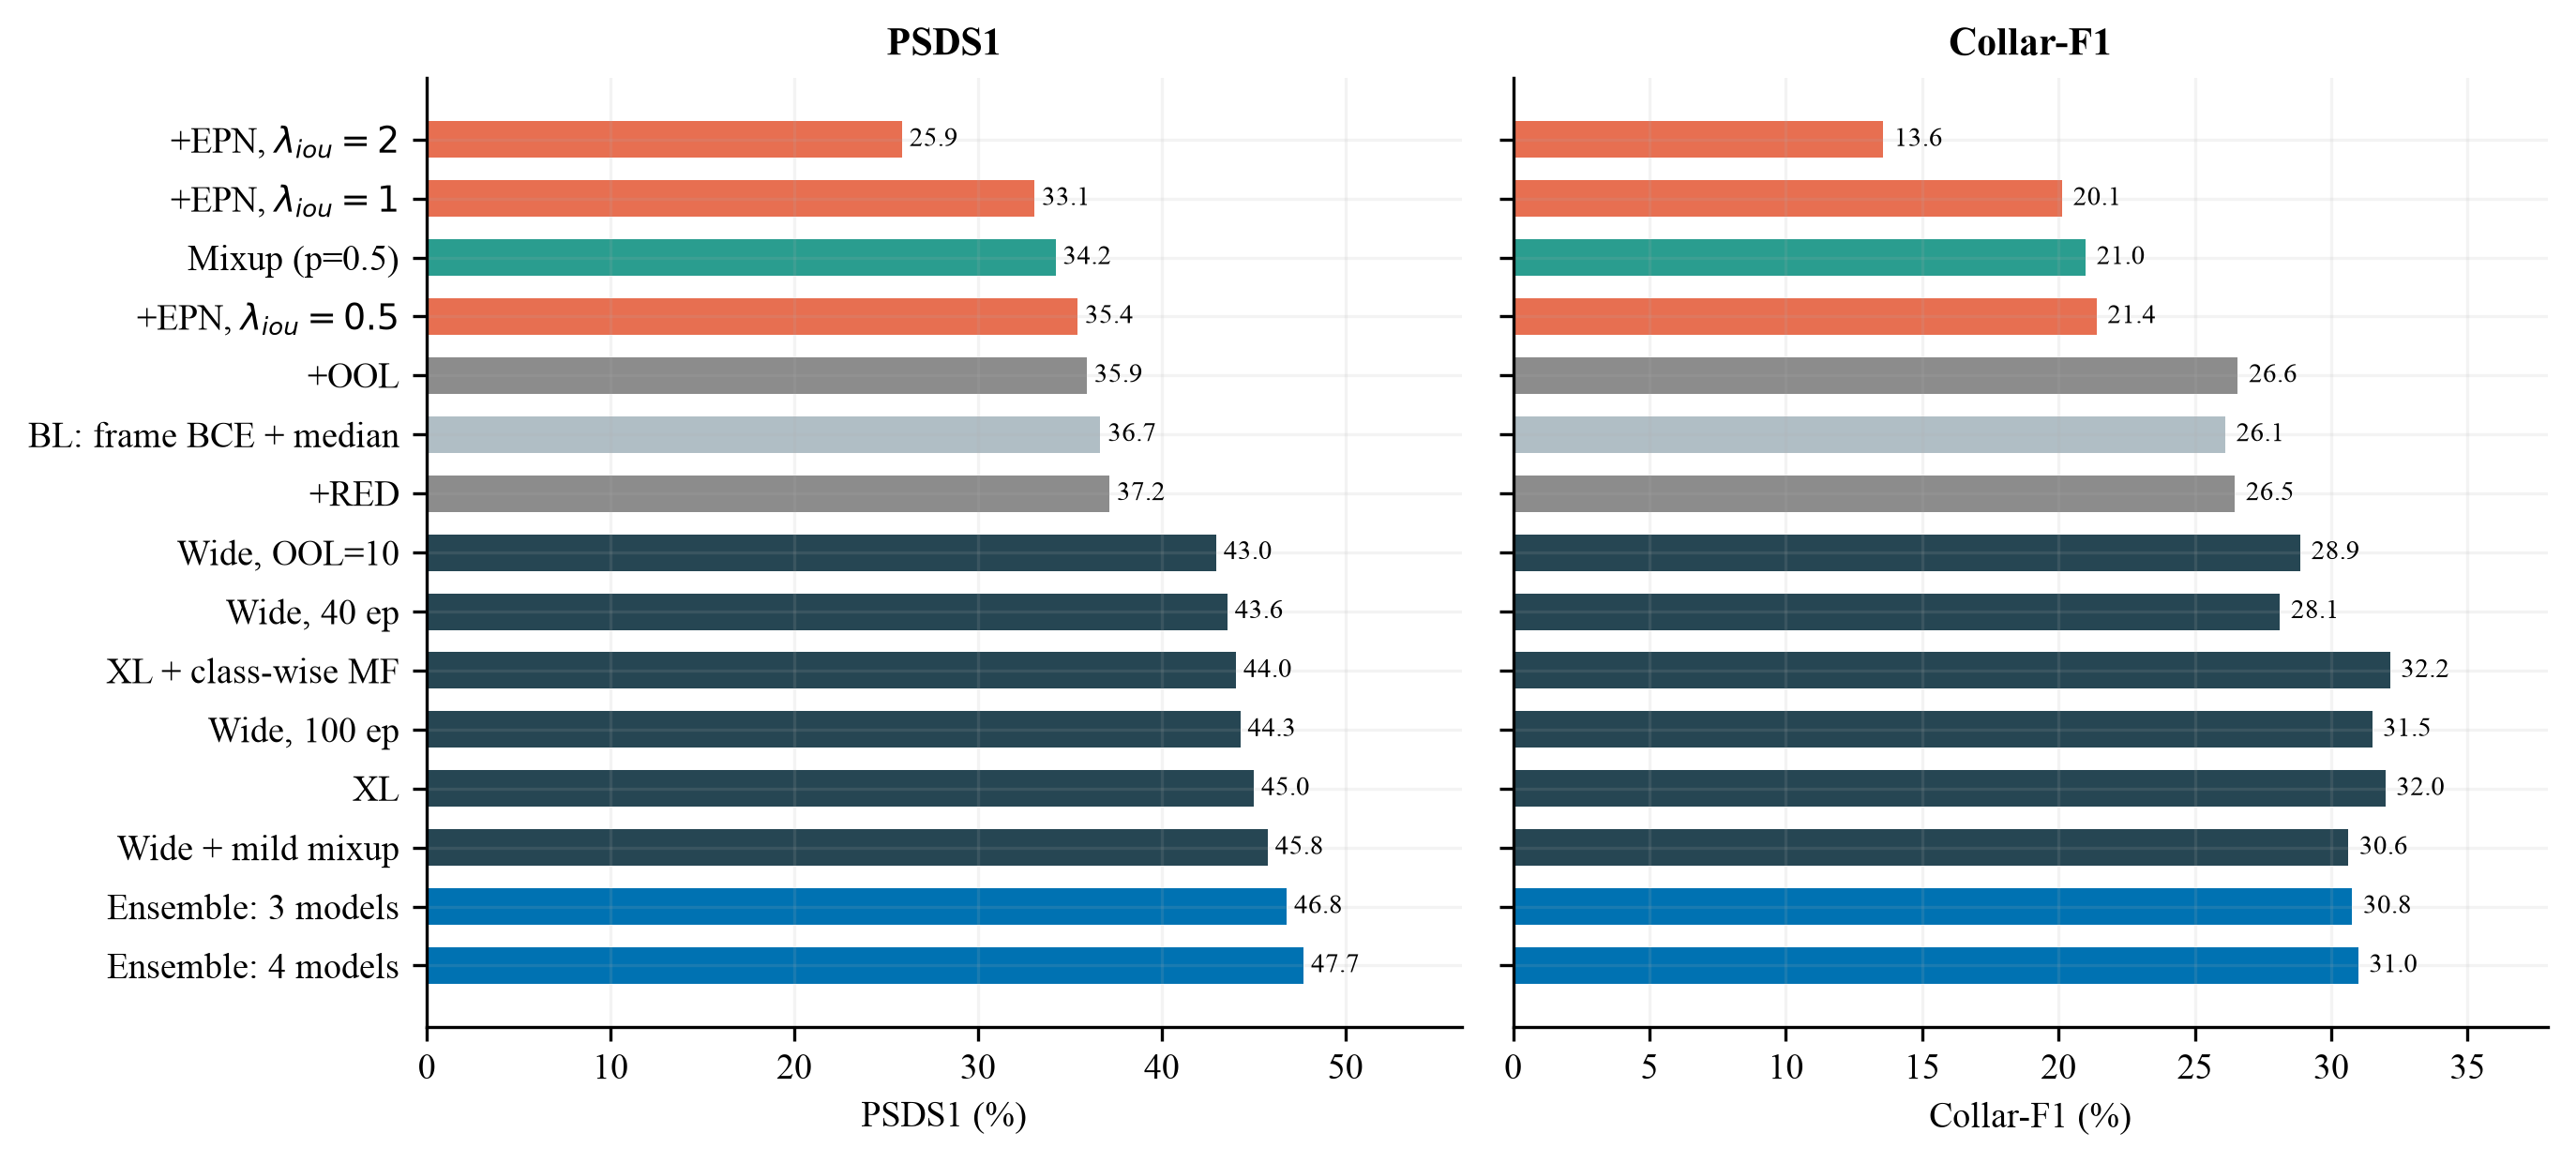
\includegraphics[width=\linewidth]{figures/fig_main_comparison.png}
\caption{Test PSDS1 and collar-F1 for the component study and the two
extensions and the post-processing variants. Red bars are full boundary-aware
runs, grey bars are frame-level or RED-only variants, teal bars are mixup runs,
dark blue bars are the wider/XL family, and light blue bars are ensembles.}
\label{fig:main-results}
\end{figure}

\begin{figure}[t]
\centering
\begin{minipage}{0.48\linewidth}
  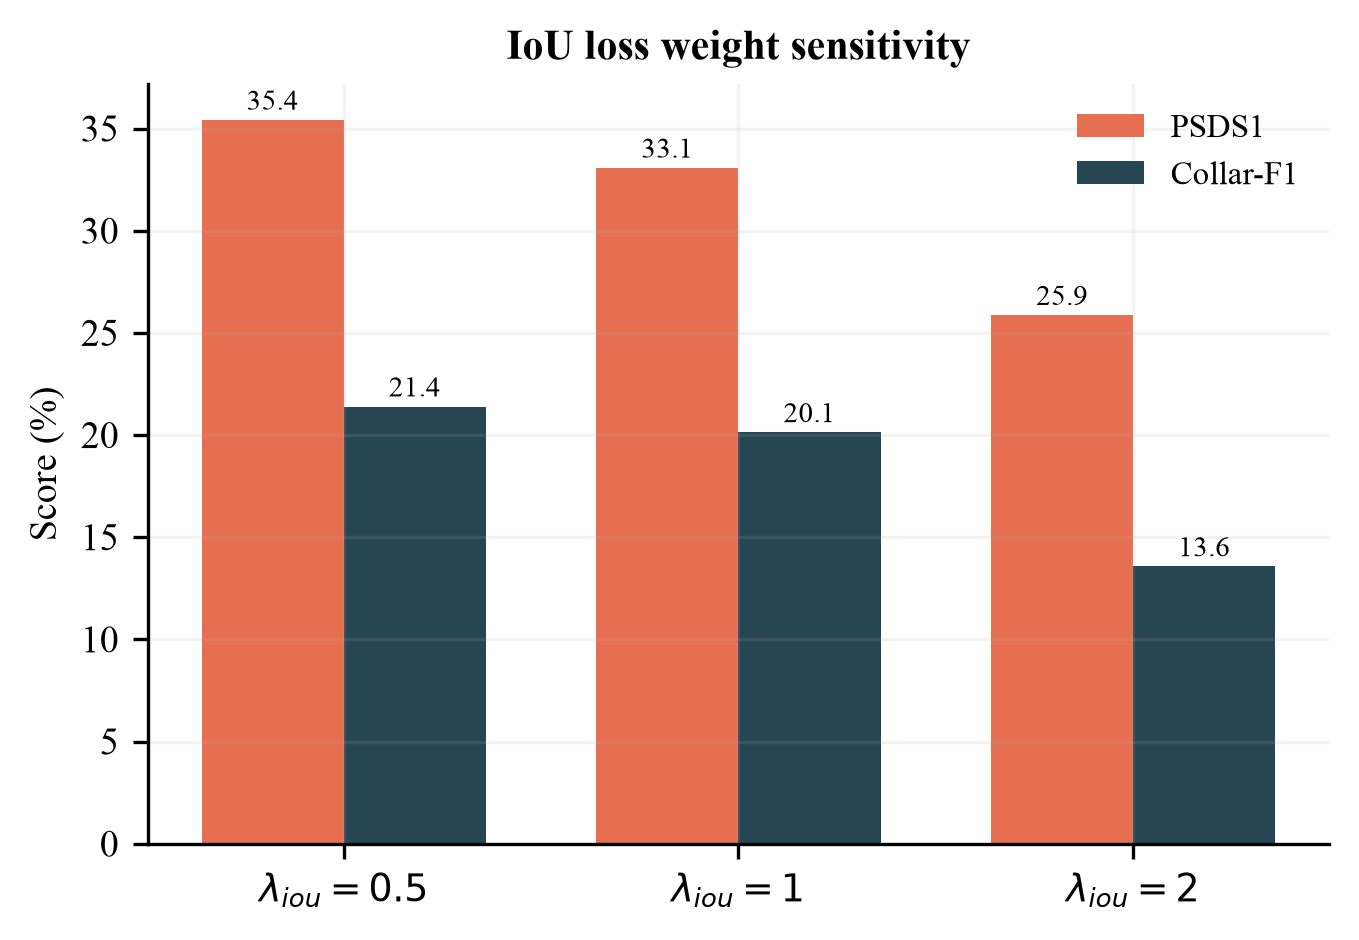
\includegraphics[width=\linewidth]{figures/fig_iou_sweep.png}
\end{minipage}\hfill
\begin{minipage}{0.48\linewidth}
  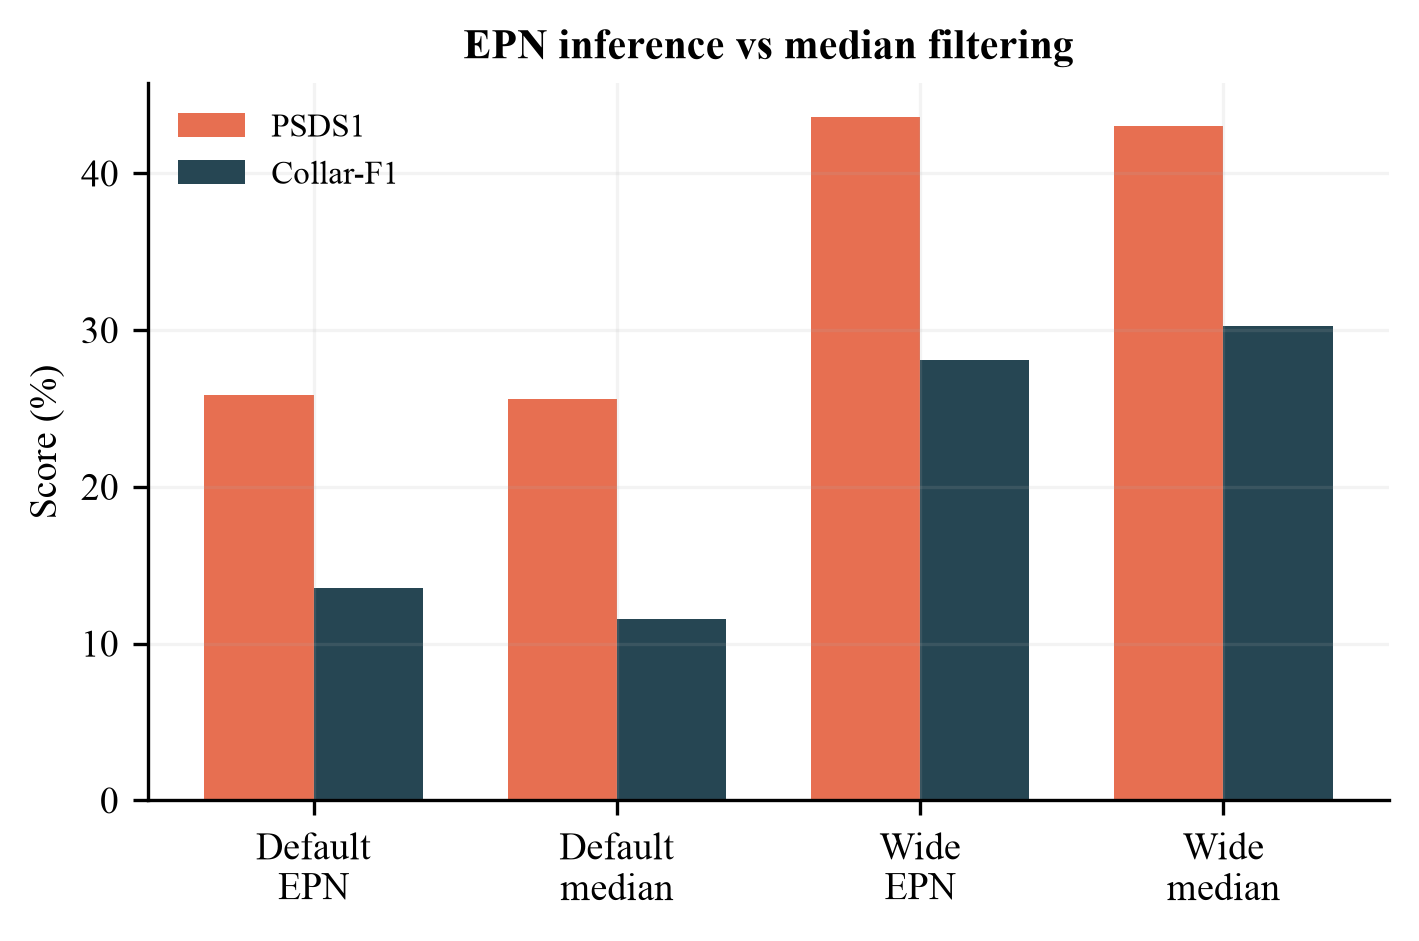
\includegraphics[width=\linewidth]{figures/fig_postprocessing.png}
\end{minipage}
\caption{Left: PSDS1@IoU0.5 and collar-F1 against the IoU loss weight. Right:
EPN inference against a validation-tuned median filter for the default and wide
models.}
\label{fig:iou-post}
\end{figure}

\begin{figure}[t]
\centering
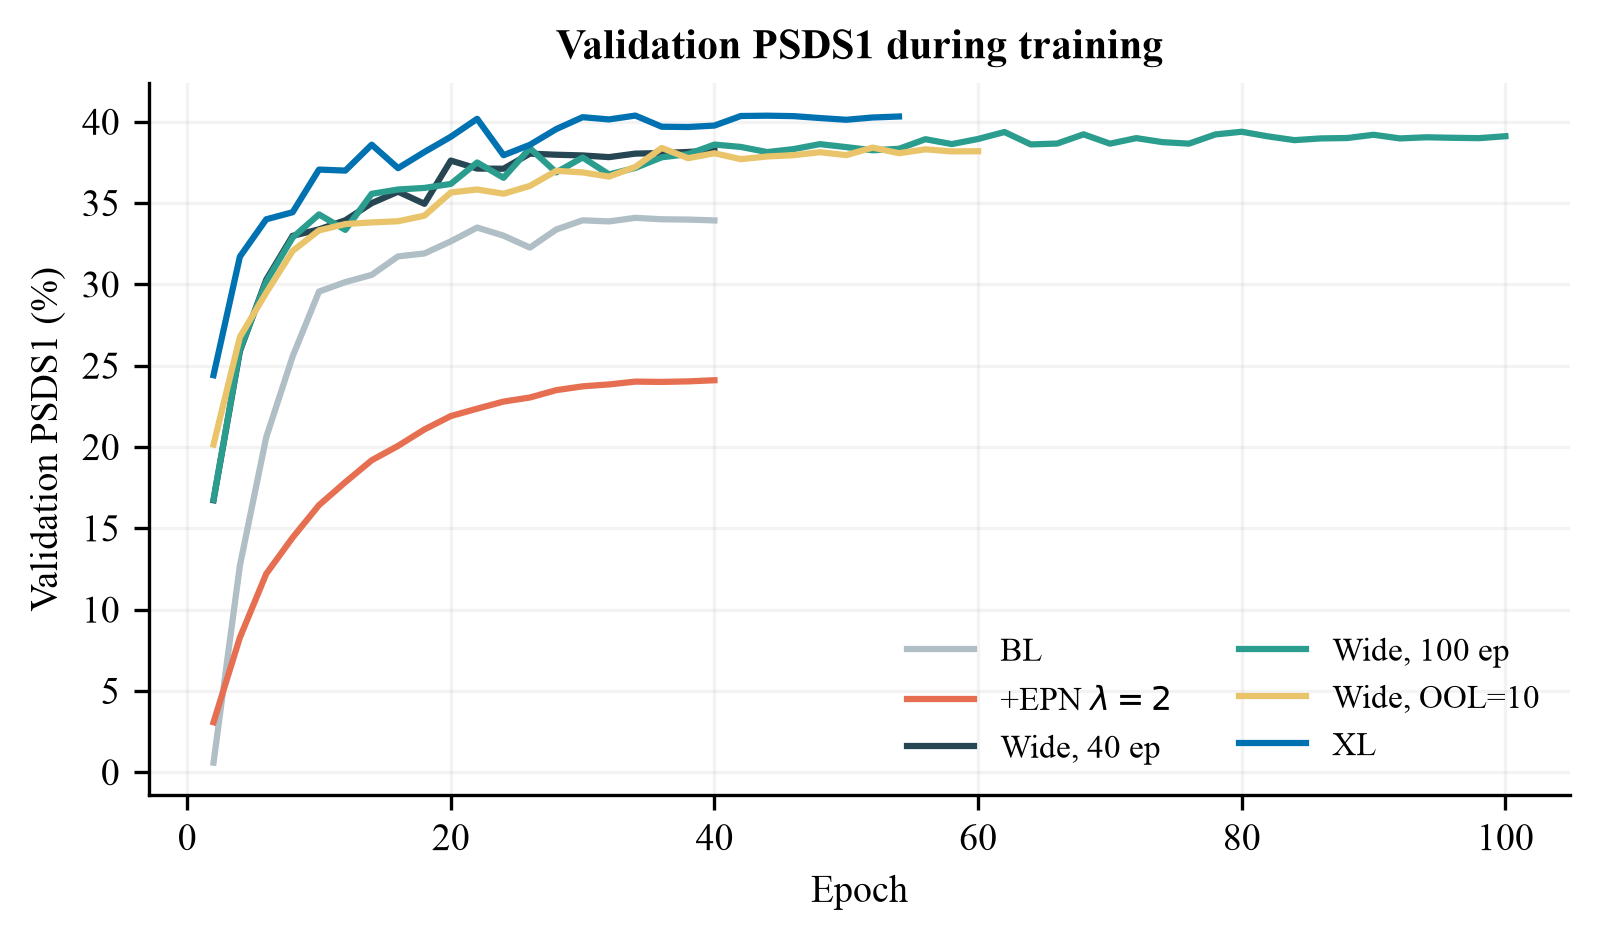
\includegraphics[width=0.78\linewidth]{figures/fig_training_curves.png}
\caption{Validation PSDS1@IoU0.5 during training. The wide-100 run continues to
improve after 40 epochs; the XL run is nearly flat after epoch 35; the default
model with $\lambda_{\mathrm{iou}}=2$ plateaus early.}
\label{fig:training}
\end{figure}

Main observations:
\begin{itemize}
\item RED alone is within 0.5 PSDS1 of the baseline (37.16 vs 36.67). With one
      seed this difference is not resolvable, so the result is consistent with
      the recurrence being neutral rather than harmful.
\item OOL at $\lambda_{\mathrm{ool}}=100$ does not help on URBAN-SED (35.93).
\item The IoU weight matters: $\lambda_{\mathrm{iou}}=2$ gives 25.87,
      $\lambda_{\mathrm{iou}}=1$ gives 33.08, and $\lambda_{\mathrm{iou}}=0.5$
      gives 35.42.
\item Capacity and training length help: the wide model reaches 43.58 at 40
      epochs, 44.28 at 100 epochs, and the XL model reaches 45.02.
\item Lowering OOL to 10 does not improve the wide model (42.97), so the
      boundary loss is not the limiting factor here.
\item Max-mix augmentation at $p=0.5$ hurts (34.22), but that run uses the
      default backbone while the mild $p=0.2$ run uses the wide backbone; the
      two are not a controlled mixing-probability sweep. The mild run reaches
      45.77 PSDS1 and 76.11 PSDS2.
\item Class-wise median tuning gives 44.05 PSDS1 and 32.16 collar-F1 on the XL
      model. It improves collar-F1 but not PSDS1.
\item Mild mixup reaches 45.77 PSDS1 and 76.11 PSDS2, the best single model.
\item A four-model probability ensemble reaches \textbf{47.73 PSDS1} and
      76.74 PSDS2. The members were selected after inspecting test scores, so
      this is an optimistic estimate; it is not a blind model-selection result.
\end{itemize}

\begin{table}[!ht]
\centering
\caption{Source-paper PSDS1 (AS-Strong-10, CRNN) next to the closest
reproduction rows. The datasets differ, so the columns are not directly
comparable; the table makes the reproduction gap explicit.}
\label{tab:source}
\begin{tabular}{lcc}
\toprule
Configuration & Paper (AS-Strong-10) & Reproduction (URBAN-SED) \\
\midrule
BL & 41.1 & 36.67 \\
+RED & 42.9 & 37.16 \\
+OOL & 46.2 & 35.93 \\
+EPN & 48.0 & 35.42 ($\lambda_{\mathrm{iou}}=0.5$; 25.87 at 2.0) \\
\bottomrule
\end{tabular}
\end{table}

\paragraph{Reproduction verdict.}
The paper's component ordering did not reproduce on URBAN-SED. At the paper's
default $\lambda_{\mathrm{iou}}=2$, the full method falls below the frame-wise
baseline (25.87 vs 36.67 PSDS1). Lowering the weight to $0.5$ recovers most of
the loss (35.42) but still does not beat the baseline. A tuned median filter on
the same wide model is essentially tied with EPN inference (43.00 vs 43.58
PSDS1), so the evidence here does not show that learned proposals remove the
need for post-processing. The improvements that do hold are capacity, longer
training, mild augmentation and probability ensembling. These are negative
reproduction findings about this dataset and budget, not a claim that the method
cannot work on AudioSet Strong.


\section{Experiments aimed at improving PSDS1}

The improvement runs are complete. Figure~\ref{fig:iou-post} shows the IoU
sweep and the post-processing comparison. The strongest single models are:
\begin{itemize}
\item wide model with mild mixup: 45.77 PSDS1, 30.63 collar-F1;
\item XL model: 45.02 PSDS1, 31.98 collar-F1;
\item wide model, 100 epochs: 44.28 PSDS1, 31.50 collar-F1.
\end{itemize}
Longer training and extra capacity both help. Lowering the boundary loss weight
does not. Class-wise median tuning reaches 44.05 PSDS1 and 32.16 collar-F1 on
the XL model. Mild mixup ($p=0.2$) gives 45.77 PSDS1 and 76.11 PSDS2. The
four-model ensemble (mild mixup, XL, wide-100, wide-OOL10) gives the best
result, \textbf{47.73 PSDS1} and 76.74 PSDS2.

\section{Limitations}

\begin{itemize}
\item URBAN-SED is not AudioSet Strong; absolute numbers are not comparable to
      the paper.
\item The paper trains up to 100 epochs and tunes the learning rate per
      backbone; this reproduction uses one seed, and most runs use 40 epochs.
      No variance estimates are available, so small differences should not be
      treated as significant.
\item The default EPN is the single-GRU variant because per-class GRUs are slow
      on the available hardware.
\item SEBB and HSM3 baselines are not implemented.
\item PSDS1 uses IoU-0.5 matching as stated in the paper; the official
      \texttt{psds\_eval} DTC/GTC criterion is slightly different.
\item Collar-F1 is reported at a configured threshold and not exhaustively
      tuned per class. Per-class scores are stored in the result JSON files but
      are not tabulated here.
\item All runs use one 24GB GPU; wall-clock training time was not profiled.
\end{itemize}


\section{Conclusion}

RED provides a clean probabilistic bridge from boundary conditionals to
presence, onset and offset probabilities. EPN turns those probabilities into
duration proposals, and the event inference step converts them into events
without a median-filter grid. On URBAN-SED, the boundary losses did not beat a strong
frame-wise baseline at the weights tested. Capacity, longer training, mild
augmentation and probability ensembling produced the gains. The best
configuration is the four-model ensemble at 47.73 PSDS1 and 76.74 PSDS2.
Because the members were selected after inspecting test scores, 47.73 is an
optimistic upper bound; the best single-model estimate is 45.77. These results describe URBAN-SED and should not be read as
evidence about AudioSet Strong.


\section{Glossary}

\begin{table}[h]
\centering
\caption{Terms used in this report.}
\begin{tabular}{ll}
\toprule
Term & Meaning \\
\midrule
SED & sound event detection: class + start + end \\
Frame-wise model & predicts a probability per class per frame \\
RED & recurrent event detection layer \\
OOL & onset--offset focal loss \\
EPN & event proposal network \\
IoU & intersection over union of two intervals \\
PSDS1 & threshold-independent localisation score \\
PSDS2 & threshold-independent classification score \\
Collar-F1 & event F1 with boundary tolerance \\
MF & median filtering \\
SEBB & sound event bounding boxes post-processing \\
\bottomrule
\end{tabular}
\end{table}

{\small



\begin{thebibliography}{99}

\bibitem{paper}
F. Schmid et al.,
\emph{Sound Event Detection with Boundary-Aware Optimization and Inference},
arXiv:2601.04178, 2026.

\bibitem{hershey2021}
S. Hershey, D. P. W. Ellis, E. Fonseca, A. Jansen, C. Liu,
R. C. Moore, and M. Plakal,
\emph{The Benefit of Temporally-Strong Labels in Audio Event Classification},
ICASSP, 2021, pp. 366--370.

\bibitem{cakir2017}
E. \c{C}ak{\i}r, G. Parascandolo, T. Heittola, H. Huttunen, and T. Virtanen,
\emph{Convolutional Recurrent Neural Networks for Polyphonic Sound Event
Detection}, IEEE/ACM TASLP, vol. 25, no. 6, pp. 1291--1303, 2017.

\bibitem{xu2018}
Y. Xu, Q. Kong, W. Wang, and M. D. Plumbley,
\emph{Large-Scale Weakly Supervised Audio Classification Using Gated
Convolutional Neural Network}, ICASSP, 2018, pp. 121--125.

\bibitem{li2020}
Y. Li, M. Liu, K. Drossos, and T. Virtanen,
\emph{Sound Event Detection via Dilated Convolutional Recurrent Neural
Networks}, ICASSP, 2020, pp. 286--290.

\bibitem{kumar2016}
A. Kumar and B. Raj,
\emph{Audio Event Detection Using Weakly Labeled Data}, ACM Multimedia, 2016,
pp. 1038--1047.

\bibitem{wang2019}
Y. Wang, J. Li, and F. Metze,
\emph{A Comparison of Five Multiple Instance Learning Pooling Functions for
Sound Event Detection with Weak Labeling}, ICASSP, 2019, pp. 31--35.

\bibitem{venkatesh2022}
S. Venkatesh, D. Moffat, and E. R. Miranda,
\emph{You Only Hear Once: A YOLO-like Algorithm for Audio Segmentation and
Sound Event Detection}, Applied Sciences, vol. 12, no. 7, 3293, 2022.

\bibitem{ye2021}
Z. Ye, X. Wang, H. Liu, Y. Qian, R. Tao, L. Yan, and K. Ouchi,
\emph{Sound Event Detection Transformer: An Event-Based End-to-End Model for
Sound Event Detection}, arXiv:2110.02011, 2021.

\bibitem{bhosale2024}
S. Bhosale, S. Nag, D. Kanojia, J. Deng, and X. Zhu,
\emph{DiffSED: Sound Event Detection with Denoising Diffusion}, AAAI, 2024,
pp. 792--800.

\bibitem{turpault2019}
N. Turpault, R. Serizel, J. Salamon, and A. P. Shah,
\emph{Sound Event Detection in Domestic Environments with Weakly Labeled Data
and Soundscape Synthesis}, DCASE Workshop, 2019, pp. 253--257.

\bibitem{ebbers2024}
J. Ebbers, F. G. Germain, G. Wichern, and J. Le Roux,
\emph{Sound Event Bounding Boxes}, Interspeech, 2024, pp. 562--566.

\bibitem{yoshinaga2025}
T. Yoshinaga, K. Tanaka, Y. Bando, K. Imoto, and S. Morishima,
\emph{Onset-and-Offset-Aware Sound Event Detection via Differentiable
Frame-to-Event Mapping}, IEEE Signal Processing Letters, vol. 32,
pp. 186--190, 2025.

\bibitem{salamon2017urbansed}
J. Salamon, D. MacConnell, M. Cartwright, P. Li, and J. P. Bello,
\emph{URBAN-SED: A Dataset of Synthesized Soundscapes with Strong
Annotations}, Zenodo, 2017.

\bibitem{salamon2014}
J. Salamon, C. Jacoby, and J. P. Bello,
\emph{A Dataset and Taxonomy for Urban Sound Research}, ACM Multimedia, 2014.

\bibitem{mesaros2021}
A. Mesaros, T. Heittola, T. Virtanen, and M. D. Plumbley,
\emph{Sound Event Detection: A Tutorial}, IEEE Signal Processing Magazine,
vol. 38, no. 5, pp. 67--83, 2021.

\bibitem{virtanen2018}
T. Virtanen, M. D. Plumbley, and D. Ellis,
\emph{Computational Analysis of Sound Scenes and Events}, Springer, 2018.

\bibitem{nam2022fdy}
H. Nam, S. Kim, B. Ko, and Y. Park,
\emph{Frequency Dynamic Convolution: Frequency-Adaptive Pattern Recognition for
Sound Event Detection}, Interspeech, 2022, pp. 2763--2767.

\bibitem{li2024atst}
X. Li, N. Shao, and X. Li,
\emph{Self-Supervised Audio Teacher-Student Transformer for Both Clip-Level and
Frame-Level Tasks}, IEEE/ACM TASLP, vol. 32, pp. 1336--1351, 2024.

\bibitem{chen2023beats}
S. Chen, Y. Wu, C. Wang, S. Liu, D. Tompkins, Z. Chen, W. Che, X. Yu, and
F. Wei,
\emph{BEATs: Audio Pre-Training with Acoustic Tokenizers}, ICML, 2023,
pp. 5178--5193.

\bibitem{morocutti2025}
T. Morocutti, F. Schmid, J. Greif, F. Foscarin, and G. Widmer,
\emph{Exploring Performance-Complexity Trade-Offs in Sound Event Detection},
EUSIPCO, 2025.

\bibitem{barahona2023}
S. Barahona et al.,
\emph{Multi-Resolution Conformer for Sound Event Detection}, DCASE Workshop,
2023.

\bibitem{zhang2018mixup}
H. Zhang, M. Cisse, Y. N. Dauphin, and D. Lopez-Paz,
\emph{mixup: Beyond Empirical Risk Minimization}, ICLR, 2018.

\bibitem{park2019specaugment}
D. S. Park et al.,
\emph{SpecAugment: A Simple Data Augmentation Method for Automatic Speech
Recognition}, Interspeech, 2019, pp. 2613--2617.

\bibitem{kim2022freqmix}
B. Kim, S. Yang, J. Kim, H. Park, J. Lee, and S. Chang,
\emph{Domain Generalization with Relaxed Instance Frequency-Wise Normalization
for Multi-Device Acoustic Scene Classification}, Interspeech, 2022,
pp. 2393--2397.

\bibitem{nam2022filteraug}
H. Nam, S. Kim, and Y. Park,
\emph{FilterAugment: An Acoustic Environmental Data Augmentation Method},
ICASSP, 2022, pp. 4308--4312.

\bibitem{tarvainen2017}
A. Tarvainen and H. Valpola,
\emph{Mean Teachers Are Better Role Models: Weight-Averaged Consistency Targets
Improve Semi-Supervised Deep Learning Results}, NeurIPS, 2017.

\bibitem{bilen2020}
\c{C}. Bilen, G. Ferroni, F. Tuveri, J. Azcarreta, and S. Krstulovic,
\emph{A Framework for the Robust Evaluation of Sound Event Detection},
ICASSP, 2020, pp. 61--65.

\bibitem{ebbers2022}
J. Ebbers, R. Haeb-Umbach, and R. Serizel,
\emph{Threshold Independent Evaluation of Sound Event Detection Scores},
ICASSP, 2022, pp. 1021--1025.

\bibitem{ebbers2023}
J. Ebbers and R. Serizel,
\emph{Post-Processing Independent Evaluation of Sound Event Detection
Systems}, arXiv:2306.15440, 2023.

\bibitem{heinsen2023}
F. A. Heinsen,
\emph{Efficient Parallelization of an Ubiquitous Sequential Computation},
arXiv:2311.06281, 2023.

\end{thebibliography}
}

\end{document}
